\documentclass[11pt]{article}
\usepackage[letterpaper,margin=1.5cm]{geometry}
\usepackage{tikz}
\usepackage{helvet}
\renewcommand{\familydefault}{\sfdefault}
\pagestyle{empty}
\setlength{\parindent}{0pt}

% ---------- Settings ----------
\newcommand{\numIDdigits}{7}      % number of digits in the student ID
\newcommand{\bubbleR}{0.2}        % bubble radius (cm)
\newcommand{\numrows}{12}
% \bubble{x}{y}{label}
\newcommand{\bubble}[3]{%
  \draw[line width=0.5pt] (#1,#2) circle (\bubbleR);
  \node[font=\fontsize{7}{7}\selectfont, text=black!100] at (#1,#2) {#3};
}

% \answerrow{x}{y}{question number}  -> choices 1,2,3,4
\newcommand{\answerrow}[3]{%
  \node[font=\small\bfseries, anchor=east] at (#1+0.8,#2) {#3.};
  \foreach \k in {1,2,3,4}{%
    \bubble{#1+0.8+0.35+0.8*\k-0.8}{#2}{\k}
  }
}

\begin{document}

\begin{center}
  {\huge\bfseries Answer Sheet}\\[2pt]
  {\small Use a dark pencil or pen. Fill bubbles completely. Erase cleanly to change an answer.}
\end{center}

\vspace{4pt}

% ---------- Handwritten name / ID ----------
\noindent

\begin{tikzpicture}
  \node[anchor=west, font=\bfseries] at (0,0) {Student Name:};
  \draw[line width=0.6pt] (3.0,-0.15) -- (12.5,-0.15);
  \node[anchor=west, font=\bfseries] at (13.2,0) {Date:};
  \draw[line width=0.6pt] (14.5,-0.15) -- (18,-0.15);
\end{tikzpicture}

\vspace{6pt}
\hrule
\vspace{6pt}

% ---------- Student ID bubbles (vertical columns, digits 0-9) ----------
\noindent
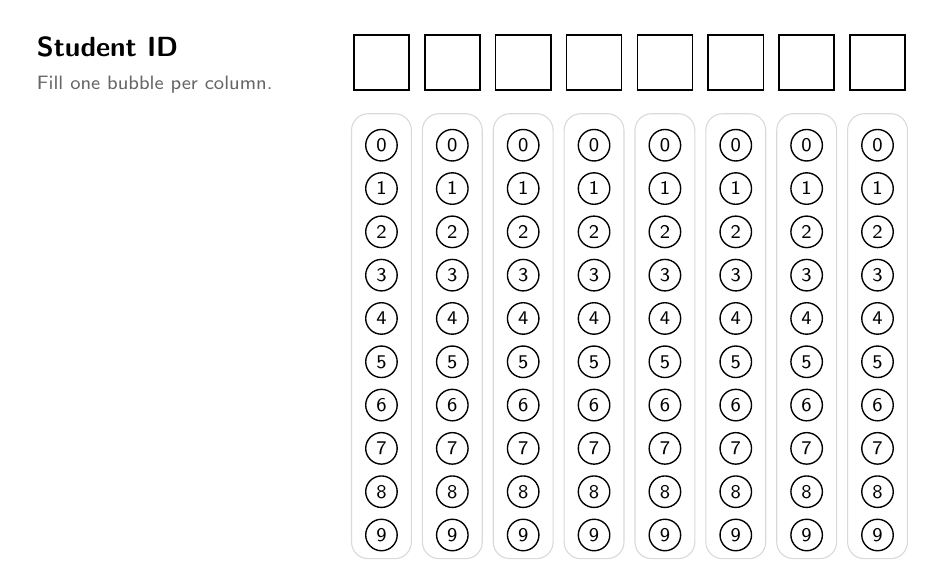
\begin{tikzpicture}
  \node[anchor=north west, font=\bfseries] at (0,0.3)
    {Student ID};
  \node[anchor=north west, font=\scriptsize, text=black!60] at (0,-0.2)
    {Fill one bubble per column.};

  % each column: header box for the digit, then 0..9 going down
  \foreach \c in {0,...,\numIDdigits}{
    \pgfmathsetmacro{\cx}{4.5+0.9*\c}
    \draw[line width=0.6pt] (\cx-0.35,0.2) rectangle (\cx+0.35,-0.5);
    \foreach \d in {0,...,9}{
      \pgfmathsetmacro{\cy}{-1.2-0.55*\d}
      \bubble{\cx}{\cy}{\d}
    }
  }
  % light column guides
  \foreach \c in {0,...,\numIDdigits}{
    \pgfmathsetmacro{\cx}{4.5+0.9*\c}
    \draw[black!15, rounded corners=6pt] (\cx-0.38,-0.8) rectangle (\cx+0.38,-6.45);
  }
\end{tikzpicture}

\vspace{4pt}
\hrule
\vspace{6pt}

% ---------- Answers ----------
\noindent
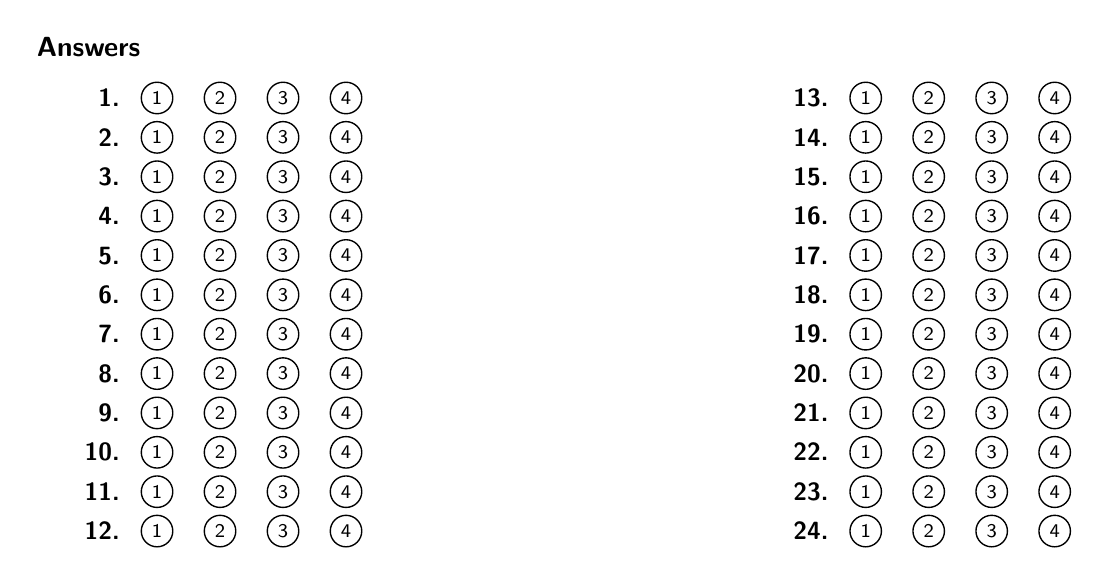
\begin{tikzpicture}
  \node[anchor=north west, font=\bfseries] at (0,0.3) {Answers};

  % Questions 1--\numrows (left), \numrows+1--2\numrows (right)
  \foreach \q in {1,...,12}{
    \pgfmathsetmacro{\y}{-0.6-0.5*(\q-1)}
    \answerrow{0.5}{\y}{\q}
    \pgfmathtruncatemacro{\r}{\q+\numrows}
    \answerrow{9.5}{\y}{\r}
  }
\end{tikzpicture}

\end{document}
